\section{Partición de Modelos de Gran Escala}
\graphicspath{ {./content/} }


\begin{frame}{Simulación en Paralelo}

Los algoritmos de simulación en paralelo requieren que:

\begin{itemize}
    \item El modelo original sea divido en $P$ submodelos.

    \item Cada submodelo sea simulado por un hilo diferente.

\end{itemize}

Para obtener una \textbf{paralelización efectiva}:

\begin{itemize}
    \item La \textbf{partición} del modelo debe ser \textbf{balanceada}.

    \item La \textbf{comunicación} entre los submodelos debe ser \textbf{minimizada}.

\end{itemize}

Llamamos a este proceso \textbf{\textit{Balance de carga estático}}.

Puede tratarse como un problema de \textbf{particionamiento de grafos}.

\end{frame}



\begin{frame}{Métodos de Particionamiento de Grafos}

    Existe diversos métodos de particionamiento de grafos:

    \begin{itemize}
        \item Los métodos actuales son sensibles al tamaño del grafo.

        \item \textbf{Métodos multinivel}: contruyen el grafo, compactan,
        optimizan y finalmente expanden el grafo.

        \item Las implementaciones de los modelos suele tener una estructura regular,
        ¿podemos aprovecharla?
    \end{itemize}

    Queremos representar el grafo computacional en forma \textbf{compacta} y particionarlo
    sin necesidad de \textbf{expandir}.

\end{frame}



\begin{frame}[fragile]{Grafo Computacional Basado en Conjuntos}

Dado el siguiente modelo Modelica:
%Lo siguiente es un fragmento de una implementación en Modelica de un modelo
%Advección-Difusión-Reacción (ADR):

  \begin{center}
    \begin{tabular}{c}
    \lstset{
        basicstyle=\scriptsize,
        emph={u},
        emphstyle=\color{red},
        morekeywords={u},
        keywordstyle=\bfseries,
        escapeinside={(*@}{@*)}
    }
      \begin{lstlisting}
          Real a[N],b[N],c[N/2],d[N/2];
          ...
          for i in 1:N loop
            der(a[i])=R*b[i];
          end for;
          for i in 1:N/2 loop
            der(c[i])=K*d[i];
          end for;
      \end{lstlisting}
    \end{tabular}
  \end{center}

  Representación del grafo computacional para las variables $c$ y $d$ con $N=10$.

  \scriptsize
  \centering
  \begin{columns}[t]
    \begin{column}{.45\linewidth}

        \begin{figure}
            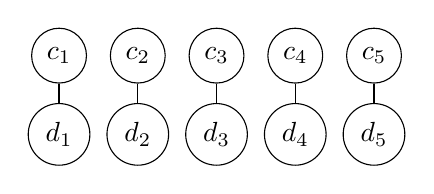
\begin{tikzpicture}[main/.style = {draw, circle}]
                \node[main] (1) [minimum height=6mm] {$c_1$};
                \node[main] (2) [minimum height=6mm,below of=1, node distance=10mm] {$d_1$}; 
                \node[main] (3) [minimum height=6mm,right of=1, node distance=10mm] {$c_2$};
                \node[main] (4) [minimum height=6mm,below of=3, node distance=10mm] {$d_2$};
                \node[main] (5) [minimum height=6mm,right of=3, node distance=10mm] {$c_3$};
                \node[main] (6) [minimum height=6mm,below of=5, node distance=10mm] {$d_3$}; 
                \node[main] (7) [minimum height=6mm,right of=5, node distance=10mm] {$c_4$};
                \node[main] (8) [minimum height=6mm,below of=7, node distance=10mm] {$d_4$}; 
                \node[main] (9) [minimum height=6mm, right of=7, node distance=10mm] {$c_5$};
                \node[main] (10) [minimum height=6mm,below of=9, node distance=10mm] {$d_5$};

                \draw (1) -- (2);
                \draw (3) -- (4);
                \draw (5) -- (6);
                \draw (7) -- (8);
                \draw (9) -- (10);

            \end{tikzpicture}
            \caption{Grafo computacional tradicional.}
        \end{figure}
    \end{column}
    \hfill
    \begin{column}{.45\linewidth}
        \vspace{-2.5em}
        \begin{figure}
            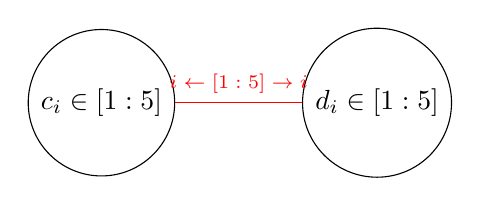
\begin{tikzpicture}[main/.style = {draw, circle}] 

                \node[main] (1) {{$c_i \in [1:5]$}};
                \node[main] (2) [right of=1, node distance=35mm] {{$d_i \in [1:5]$}};

                \draw[color=red] (1) -- (2) node [midway, above] {\scriptsize{$i \gets [1:5] \to i$}};
                % \draw[loop above, color=black] (2) to node[near start, above] {\scriptsize{$i + 1 \gets [2:9] \to i$}} (2);

            \end{tikzpicture}
            \caption{Grafo computacional basado en conjuntos.}
        \end{figure}
    \end{column}
  \end{columns}

\end{frame}

\begin{frame}{Fase de Optimización}

    Sean $\color{black}A^*$ y $\color{black}B^*$ la partición de un conjunto con $edgeCut$ mínimo.

    Sean $\color{black}A$ y $\color{black}B$ dos particiones iniciales. Existen subconjuntos
    $\color{black}X \in A$ y $\color{black}Y \in B$ tales que:

  \begin{figure}
  \centering
  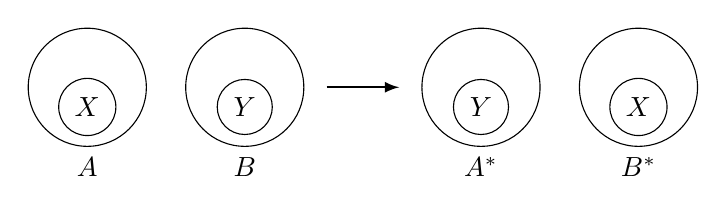
\begin{tikzpicture}[main/.style = {draw, circle}, minimum height=5mm] 
      \node[main] (A) [minimum height=15mm, label=below:$\color{black}A$] {};
      \node[main] (X) [below of=A, node distance=2.5mm] {$\color{black}X$}; 
  
      \node[main] (B) [right of=A, node distance=20mm, minimum height=15mm, label=below:$\color{black}B$] {};
      \node[main] (Y) [below of=B, node distance=2.5mm] {$\color{black}Y$}; 
  
  
      \node[main] (A1) [right of=B, node distance= 30mm, minimum height=15mm, label=below:$\color{black}A^*$] {};
      \node[main] (Y1) [below of=A1, node distance=2.5mm] {$\color{black}Y$};
  
      \node[main] (B1) [right of=A1, node distance=20mm, minimum height=15mm, label=below:$\color{black}B^*$] {};
      \node[main] (X1) [below of=B1, node distance=2.5mm] {$\color{black}X$}; 
  
      \draw [-latex,thick,shorten >=8pt,shorten <=8pt] (B) edge (A1);
  \end{tikzpicture}
  
  $\color{black} A^* = A - X + Y$
  
  $\color{black}B^* = B - Y + X$
  \caption{Descripción gráfica de la fase de optimización.}
  \end{figure}
    
\end{frame}



\begin{frame}[fragile]{Fase de Optimización}

  \begin{columns}
    \begin{column}{0.6\linewidth}
        \begin{figure}
            \begin{center}
                    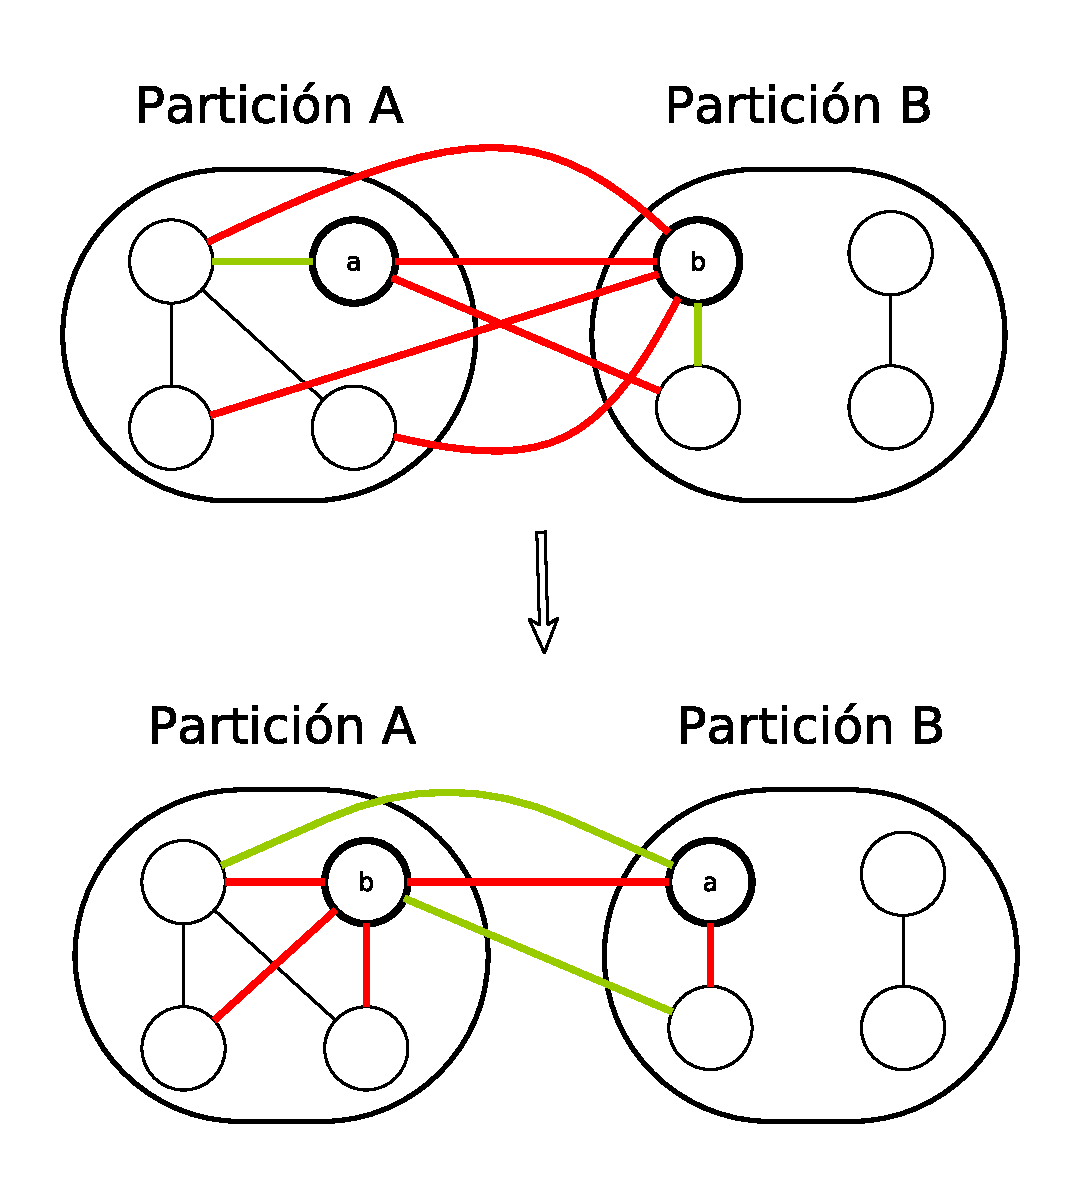
\includegraphics[width=0.75\textwidth]{graph_partition_gropup.pdf}
            \end{center}

            \scriptsize
            \color{red} --- \color{black} Comunicación externa de los nodos \textbf{a} y \textbf{b}.\\
            \color{green} --- \color{black} Comunicación interna de los nodos \textbf{a} y \textbf{b}.
            \caption{Descripción gráfica del cálculo de la ganancia.}
        \end{figure}
    \end{column}

    \hfill

    \begin{column}{0.35\linewidth}
        \footnotesize
          $D_a = \#EC_a - \#IC_a = 1$\\
          $D_b = \#EC_b - \#IC_b = 3$\\
          $gain_{ab} = D_a + D_b - 2c_{ab} = 2$\\
          $c_{ab} \text{ es la comunicación entre}$\\
          $\text{los nodos a y b.}$
    \end{column}
  \end{columns}
\end{frame}



\begin{frame}{Optimización de Grafos Basados en Conjuntos}

    \begin{columns}[T]
        \begin{column}{0.65\textwidth}
            \begin{figure}
                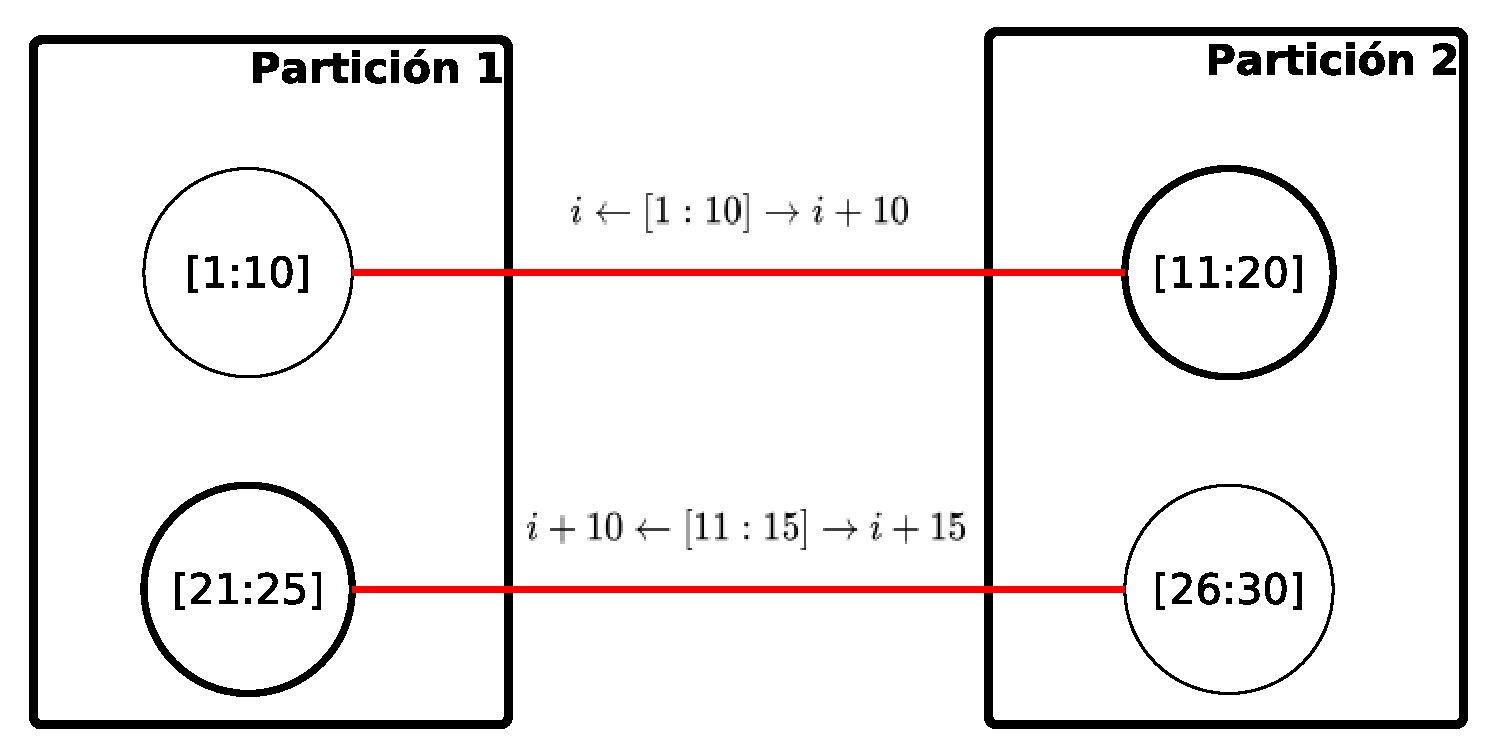
\includegraphics[width=1\textwidth]{graph_compact.pdf}
                \caption{Representación gráfica del particionamiento de un
                Grafo Computacional Basado en Conjuntos.}
            \end{figure}
        \end{column}

        \begin{column}{0.35\textwidth}
          % \begin{center}
            \vspace{2em}
            \footnotesize
            Sean $a = \{[[11:15]]\}$ y $ b = \{[21:25]\}$:
            \vspace{0.5em}

              $D_a = \#EC_a - \#IC_a = 5$\\
              \vspace{0.5em}
              $D_b = \#EC_b - \#IC_b = 5$\\
              \vspace{0.5em}
              $gain_{ab} = D_a + D_b - 2c_{ab} = 10$\\
              \vspace{0.5em}
              $c_{ab} \text{ es la comunicación entre}$\\
              $\text{los nodos a y b.}$
          % \end{center}
        \end{column}
    \end{columns}
\end{frame}



\begin{frame}{Optimización de Grafos Basados en Conjuntos}
    \begin{figure}
        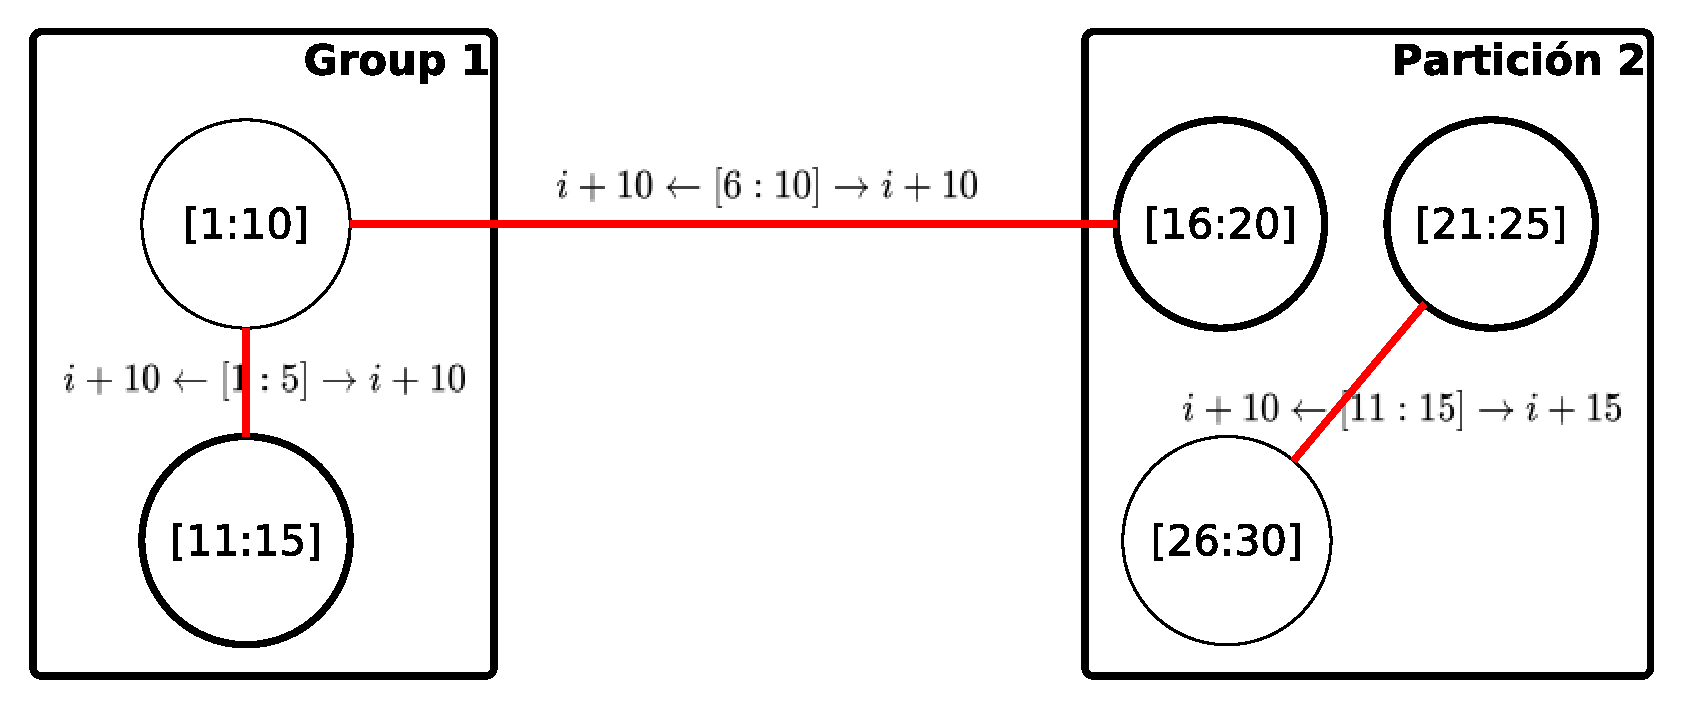
\includegraphics[width=0.75\textwidth]{graph_compact_2.pdf}
        \caption{Representación gráfica del particionamiento tras un paso
        de optimización.}
    \end{figure}
\end{frame}



\section{Resultados}


\begin{frame}{Métricas de particionado}

    Métricas de calidad de particionado:
    
    \begin{itemize}
        \item \textbf{Edge-Cut}.
    
        \item \textbf{Volumen de comunicación total}.
    
        \item \textbf{Volumen de comunicación máximo}.
    
        \item \textbf{Desbalance máximo}.
    \end{itemize}

        Métricas de rendimiento:
    
    \begin{itemize}
        \item{\textbf{Tiempo de Inicialización}}.
    
        \item{\textbf{Tiempo de Particionado}}.
    \end{itemize}

    \vspace{1em}

    METIS implementa de métodos multinivel y será utilizado para comparar los resultados
    obtenidos.
    
\end{frame}



\begin{frame}{Modelo ADR}

    Dado que las variables que comunican datos entre las distintas particiones son $u[i]$ con $u[i-1]$ para
    un determinado rango. El $edgeCut$ es igual a 3, pues es la arista
    que comunica los dos nodos adyacentes entre particiones independientemente del tamaño.

    \begin{table}[H]
        \centering
        \resizebox{\textwidth}{!}{\begin{tabular}{*{7}{c}}
        \toprule
        \multicolumn{1}{c}{\textbf{Particionador}} & \multicolumn{1}{c}{\textbf{Inicialización}} & \multicolumn{1}{c}{\textbf{Particionado}} & \multicolumn{1}{c}{\textbf{Edge}} & \multicolumn{1}{c}{\textbf{Communication}} & \multicolumn{1}{c}{\textbf{Maximum}} & \multicolumn{1}{c}{\textbf{Maximum}} \\

        \multicolumn{1}{c}{\textbf{ }} & \multicolumn{1}{c}{\textbf{(ms)}} & \multicolumn{1}{c}{\textbf{(ms)}} & \multicolumn{1}{c}{\textbf{cut}} & \multicolumn{1}{c}{\textbf{volume}} & \multicolumn{1}{c}{\textbf{volume}} & \multicolumn{1}{c}{\textbf{imbalance}} \\

        \midrule
        SBG-Partitioner & $0,4$ & $5,31$ & $3$ & $6$ & $2$ & $0$ \\
        METIS & $2,9$ & $1,2$ & $3$ & $6$ & $2$ & $1,28\mathrm{e}{2}$ \\
        % Scotch & $3$ & $2$ & $3$ & $6$ & $2$ & $9,2\mathrm{e}{-3}$ \\
        \bottomrule
        \end{tabular}}
        \caption{Modelo con tamaño 10000}
    \end{table}

    \begin{table}[H]
        \centering

        \resizebox{\textwidth}{!}{
        \begin{tabular}{*{7}{c}}
        \toprule
        \multicolumn{1}{c}{\textbf{Particionador}} & \multicolumn{1}{c}{\textbf{Inicialización}} & \multicolumn{1}{c}{\textbf{Particionado}} & \multicolumn{1}{c}{\textbf{Edge}} & \multicolumn{1}{c}{\textbf{Communication}} & \multicolumn{1}{c}{\textbf{Maximum}} & \multicolumn{1}{c}{\textbf{Maximum}} \\

        \multicolumn{1}{c}{\textbf{ }} & \multicolumn{1}{c}{\textbf{(ms)}} & \multicolumn{1}{c}{\textbf{(ms)}} & \multicolumn{1}{c}{\textbf{cut}} & \multicolumn{1}{c}{\textbf{volume}} & \multicolumn{1}{c}{\textbf{volume}} & \multicolumn{1}{c}{\textbf{imbalance}} \\

        \midrule
        SBG-Partitioner & $0,5$ & $5,51$ & $3$ & $6$ & $2$ & $0$ \\
        METIS & $26$ & $12$ & $3$ & $6$ & $2$ & $1,76\mathrm{e}{-2}$ \\
        % Scotch & $26$ & $10$ & $3$ & $6$ & $2$ & $1,8\mathrm{e}{-3}$\\
        \bottomrule
        \end{tabular}}
        \caption{Modelo con tamaño 100000}
    \end{table}

\end{frame}



\begin{frame}{Modelo Aires Acondicionados con Controlador}

    Este modelo representa una población de aires acondicionados, divida por secciones,
    cada sección conectada a un controlador parcial, y estos conectados a un controlador
    centralizado.

    \begin{table}[H]
        \centering
        \resizebox{\textwidth}{!}{\begin{tabular}{*{7}{c}}
        \toprule
        \multicolumn{1}{c}{\textbf{Particionador}} & \multicolumn{1}{c}{\textbf{Inicialización}} & \multicolumn{1}{c}{\textbf{Particionado}} & \multicolumn{1}{c}{\textbf{Edge}} & \multicolumn{1}{c}{\textbf{Communication}} & \multicolumn{1}{c}{\textbf{Maximum}} & \multicolumn{1}{c}{\textbf{Maximum}} \\
    
        \multicolumn{1}{c}{\textbf{ }} & \multicolumn{1}{c}{\textbf{(ms)}} & \multicolumn{1}{c}{\textbf{(ms)}} & \multicolumn{1}{c}{\textbf{cut}} & \multicolumn{1}{c}{\textbf{volume}} & \multicolumn{1}{c}{\textbf{volume}} & \multicolumn{1}{c}{\textbf{imbalance}} \\
    
        \midrule
        SBG-Partitioner & $2$ & $7275$ & $75004$ & $150005$ & $74999$ & $1,3\mathrm{e}{-5}$ \\
        METIS & $182$ & $105$ & $149925$ & $149927$ & $75004$ & $1,3\mathrm{e}\mathrm{-5}$ \\
        \bottomrule
        \end{tabular}}
        \caption{Modelo con tamaño 100000}
    \end{table}

    \begin{table}[H]
        \centering
        \resizebox{\textwidth}{!}{\begin{tabular}{*{7}{c}}
        \toprule
        \multicolumn{1}{c}{\textbf{Particionador}} & \multicolumn{1}{c}{\textbf{Inicialización}} & \multicolumn{1}{c}{\textbf{Particionado}} & \multicolumn{1}{c}{\textbf{Edge}} & \multicolumn{1}{c}{\textbf{Communication}} & \multicolumn{1}{c}{\textbf{Maximum}} & \multicolumn{1}{c}{\textbf{Maximum}} \\
    
        \multicolumn{1}{c}{\textbf{ }} & \multicolumn{1}{c}{\textbf{(ms)}} & \multicolumn{1}{c}{\textbf{(ms)}} & \multicolumn{1}{c}{\textbf{cut}} & \multicolumn{1}{c}{\textbf{volume}} & \multicolumn{1}{c}{\textbf{volume}} & \multicolumn{1}{c}{\textbf{imbalance}} \\
    
        \midrule
        SBG-Partitioner & $3$ & $7360$ & $750004$ & $1500005$ & $749999$ & $1.3\mathrm{e}{-6}$ \\
        METIS & $14741$ & $1501$ & $1500003$ & $1500004$ & $749973$ & $6,5\mathrm{e}\mathrm{-5}$ \\
        \bottomrule
        \end{tabular}}
        \caption{Modelo con tamaño 1000000}
    \end{table}

\end{frame}



\section{Trabajo Futuro}



\begin{frame}{Trabajo Futuro}

    \begin{itemize}
        \item Implementación:
    
        \begin{itemize}
            \item Actualizar librería SBG a su última versión.
            \item Evitar recomputar conexiones innecesariamente (estado global).
            \item Posibilitar el desbalance de particiones.
        \end{itemize}

        \item Mejorar $KL-SBG$ para $N$ particiones usando las componentes conexas
        del grafo, no sólo aristas individuales.
    
        \item Implementar algoritmos de balance de carga semi-estático y dinámico
        usando SBG.
    \end{itemize}

\end{frame}